\documentclass[9pt, aspectratio=169]{beamer}

\usetheme{metropolis}
\setbeamertemplate{itemize items}{\faAngleRight}

\metroset{titleformat=smallcaps,block=fill,numbering=counter,progressbar=frametitle,sectionpage=none}
\setbeamersize{text margin left=5mm,text margin right=5mm} 
% \input{embed_video}
\usepackage{fontspec,minted}
\usepackage[scale=1]{ccicons}
\usepackage{metalogo}
\usepackage{xcolor,colortbl}
\usepackage{multicol,multirow,booktabs}
\usepackage{appendixnumberbeamer}
\usepackage{graphicx}
\usepackage{mismath}
\usepackage{bm}
\usepackage{fontawesome5}
\usepackage{csquotes}
\usepackage[backend=biber, natbib, sorting=nyt, doi=true, url=false, url=false, isbn=false, maxbibnames=10]{biblatex}
\addbibresource{../utils/refs.bib}

\usepackage[spanish, es-nodecimaldot]{babel}
\deftranslation[to=spanish]{Definition}{Definición}
\deftranslation[to=spanish]{Theorem}{Teorema}
\deftranslation[to=spanish]{Example}{Ejemplo}

\usepackage{mathtools, mathrsfs}
\usefonttheme{professionalfonts}
\usepackage{textcomp, wasysym}

\setsansfont[BoldFont={Iwona Heavy}, Numbers={Lining, Proportional}]{Iwona Light}
\setmonofont[Scale=MatchLowercase]{Hack Nerd Font Mono}

\setbeamercolor{alerted text}{fg=red,bg=black!2}
\setbeamercolor{progress bar}{fg=red,bg=red!2}
\setbeamertemplate{itemize item}{\faCaretRight}
\setbeamertemplate{itemize subitem}{ \faAngleRight}
\setbeamertemplate{blocks}[shadow=false]
\setbeamercolor{block title}{bg=black!30,fg=red}
\setbeamercolor{block body}{bg=black!20,fg=black}
\setbeamertemplate{theorem begin}
{%
\begin{\inserttheoremblockenv}
{%
\inserttheoremheadfont
%{Teorema:}
\inserttheoremname
\ifx\inserttheoremaddition\@empty\else\ : \inserttheoremaddition\fi%
\inserttheorempunctuation
}%
}
\setbeamertemplate{theorem end}{\end{\inserttheoremblockenv}}
\makeatother


 
\usepackage{gensymb,amssymb}
\usepackage{siunitx}
\DeclareSIUnit{\nada}{\relax}
\usepackage{upquote}
\usepackage{cancel}
\usepackage{algpseudocode}
\algrenewcommand\algorithmicrequire{\textbf{Requiere}}
\algrenewcommand\algorithmicensure{\textbf{Devuelve}}
\setbeamertemplate{blocks}[shadow=false]

\newcommand{\cx}{\column{0.5\textwidth}}
\newcommand{\cw}[1]{\column{#1\textwidth}}

\author{Manuel Carlevaro}
\date{{\tiny Departamento de Ingeniería Mecánica \\
             Grupo de Materiales Granulares - UTN FRLP \\
             manuel.carlevaro@gmail.com }}
\institute{
  \vspace{6em}
  \centering
  {\tiny
  Cálculo Avanzado \enspace • \enspace 2025 \\
    \faLinux \- $\cdot$ \- \fontspec{TeX Gyre Pagella}\XeLaTeX \- $\cdot$ \- \ccbysa }
}

%% Operadores
\DeclareMathOperator{\sen}{sen}
\DeclareMathOperator{\senc}{senc}
\DeclareMathOperator{\sign}{sign}
\DeclareMathOperator{\Tr}{Tr}
\DeclareMathOperator{\rg}{rg}
\DeclareMathOperator{\cond}{cond}
\newcommand{\T}[1]{\underline{\bm{#1}}}
\newcommand{\uvec}[1]{\hat{\bm{#1}}}

\usepackage{hyperref}
\hypersetup{
    colorlinks,
    citecolor=blue,
    filecolor=black,
    linkcolor=blue,
    urlcolor=blue
}
\urlstyle{same}

%% Códigos
\usepackage{minted}
\newminted[cpp]{cpp}{linenos,fontsize=\footnotesize,frame=lines,numbersep=4pt}
\newmintedfile[cppcode]{cpp}{linenos,fontsize=\footnotesize,frame=lines,numbersep=4pt}
\newcommand{\mic}[1]{\mintinline{C++}{#1}}

\newminted[py]{python}{linenos,fontsize=\footnotesize,frame=lines,numbersep=4pt}
\newminted[pyc]{pycon}{linenos,fontsize=\footnotesize,frame=lines,numbersep=4pt} % Consola de Python
\newminted[ipy3]{ipython3}{linenos,fontsize=\footnotesize,frame=lines,numbersep=4pt} % Consola de iPython3
\newmintedfile[pycode]{python}{linenos,fontsize=\footnotesize,frame=lines,numbersep=4pt}

\newmintedfile[makef]{basemake}{linenos,fontsize=\footnotesize,frame=lines,numbersep=4pt}
\definecolor{bg}{RGB}{22,43,58}
\newminted[shell]{console}{linenos=false,fontsize=\footnotesize,breaklines=true, frame=single} % Linea de comandos
\renewcommand\listingscaption{Código}

\makeatletter
\AtBeginEnvironment{minted}{\dontdofcolorbox}
\def\dontdofcolorbox{\renewcommand\fcolorbox[4][]{##4}}
\makeatother

% uso:
% Ejemplo de uso explícito:
% \begin{py}
% >>> list("abcd")
% ['a', 'b', 'c', 'd']
% \end{py}
% 
% Ahora ejemplo de código en file:
% \pycode{Chapters/intro/code/hola.py}
% 
% También se puede poner un sector del file:
% \pycode[firstline=6, lastline=7]{Chapters/intro/code/hola.py}
% 
% También se puede poner código \textit{inline}: \mip{print('¡Hola mundo!')} y en una sola línea:
% \slp|if __name__ == '__main__')|
% 
% Por último, se puede poner el código en un entorno \textit{float}, esto es, como las tablas y las figuras, con un caption y un label para luego hacer referencias, como por ejemplo al Código \ref{code:hola}.


\usepackage{tikz}
\usetikzlibrary{shapes,shadows,arrows,positioning,matrix,chains,backgrounds,fit}

\tikzset{
    %Define standard arrow tip
    >=stealth',
    %Define style for boxes
    obj/.style={
           rectangle,
           rounded corners,
           draw, very thick,
           text width=10em, fill=green!20,
           minimum height=2em,
           text centered, drop shadow},
    proc/.style={
	    rectangle, rounded corners,
	    draw,fill=red!50,very thick,
	    text width=8em,minimum height=2em,
	    text centered, drop shadow},
    % Define arrow style
    pil/.style={
           ->,
           thick,
           shorten <=2pt,
           shorten >=2pt,}
}

\setbeamertemplate{bibliography item}{%
  \ifboolexpr{ test {\ifentrytype{book}} or test {\ifentrytype{mvbook}}
    or test {\ifentrytype{collection}} or test {\ifentrytype{mvcollection}}
    or test {\ifentrytype{reference}} or test {\ifentrytype{mvreference}} }
    {\setbeamertemplate{bibliography item}{\faBook}}
    {\ifentrytype{online}
            {\setbeamertemplate{bibliography item}{\faGlobe}}
   {\setbeamertemplate{bibliography item}{\faFileText}}}%
  \usebeamertemplate{bibliography item}}

\defbibenvironment{bibliography}
  {\list{}
     {\settowidth{\labelwidth}{\usebeamertemplate{bibliography item}}%
      \setlength{\leftmargin}{\labelwidth}%
      \setlength{\labelsep}{\biblabelsep}%
      \addtolength{\leftmargin}{\labelsep}%
      \setlength{\itemsep}{\bibitemsep}%
      \setlength{\parsep}{\bibparsep}}}
  {\endlist}
  {\item}
\newcommand{\bcite}[1]{\citeauthor{#1}, \citetitle{#1} (\citeyear{#1})}

\addbibresource{../utils/refs.bib}

\title{Resolución de problemas de valor inicial}
\subtitle{}

%%%%
% Bibliografía
% Burden y Faires
% Mathews y Fink
%%%%

\begin{document}
\maketitle

\begin{frame}{Dos abordajes:}
\begin{columns}[]
    \column{0.4\textwidth}
    \begin{center}
      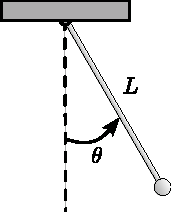
\includegraphics[width=0.6\textwidth]{figs/pendulo.pdf}
    \end{center}
    \column{0.5\textwidth}
    \[ \frac{d^2 \theta}{dt^2} + \frac{g}{L} \sen \theta = 0, \qquad \theta(t_0) = \theta_0, \qquad \theta  (t_0) = \theta \]
\end{columns}
\end{frame}


\begin{frame}
\begin{columns}[t]
\cw{0.45}
\textbf{Problema de valor inicial:}
\vspace{1em}

\[ \begin{system}
    y'(t) = f[t, y(t)], \quad t_0 \leq t \leq T \\
    y(t_0) = y_0
\end{system} \] \pause 
\vspace{1em}
\begin{definition}[Condición de Lipschitz]
    Una función $f(t, y)$ satisface una \textbf{condición de Lipschitz} en la variable $y$, y en un conjunto $D \in \R^2$ si existe una constante $L > 0$ tal que 
    \[ \abs{f(t, y_1) - f(t, y_2)} \leq L \abs{y_1 - y_2} \]
    siempre que $(t, y_1)$ y $(t, y_2)$ estén en $D$. La constante $L$ se llama \textbf{constante de Lipschitz} para $f$.
\end{definition} \pause

\cw{0.45}
\textbf{Ejemplo:} mostrar que $f(t, y) = t \abs{y}$ satisface una condición de Lipschitz en el intevalo $D = \{ (t, y) \, | \, 1 \leq t \leq2 \text{ y } -3 \leq y \leq 4\}$:

Para cada par de puntos $(t, y_1)$ y $(t, y_2)$ en $D$, tenemos:
\begin{align*}
    \abs{f(t, y_1) - f(t, y_2)} &= \abs{t \abs{y_1} - t \abs{y_2}} \\
                                &= \abs{t} \abs{\abs{y_1} - \abs{y_2}} \\
                                &\leq 2 \abs{y_1 - y_2}
\end{align*}
$f$ satisface una condición de Lipschitz sobre $D$ con $L = 2$ (menor valor posible). Por ejemplo:
\[ \abs{f(2, 1) - f(2, 0)} = \abs{2 - 0} = 2 \abs{1 - 0} \]
\end{columns}
\end{frame}

\begin{frame}
\begin{columns}
\cx 
\begin{definition}[Conjunto convexo]
    Un conjunto $D \in \R^2$ se dice que es \textbf{convexo} si, dados $(t_1, y_1)$ y $(t_2, y_2)$ pertenecientes a $D$, entonces
    \[ [(1 - \lambda) t_1 + \lambda t_2, (1 - \lambda) y_1 + \lambda y_2] \in D \;  \forall \lambda \in [0, 1] \]
\end{definition}
\begin{center}
    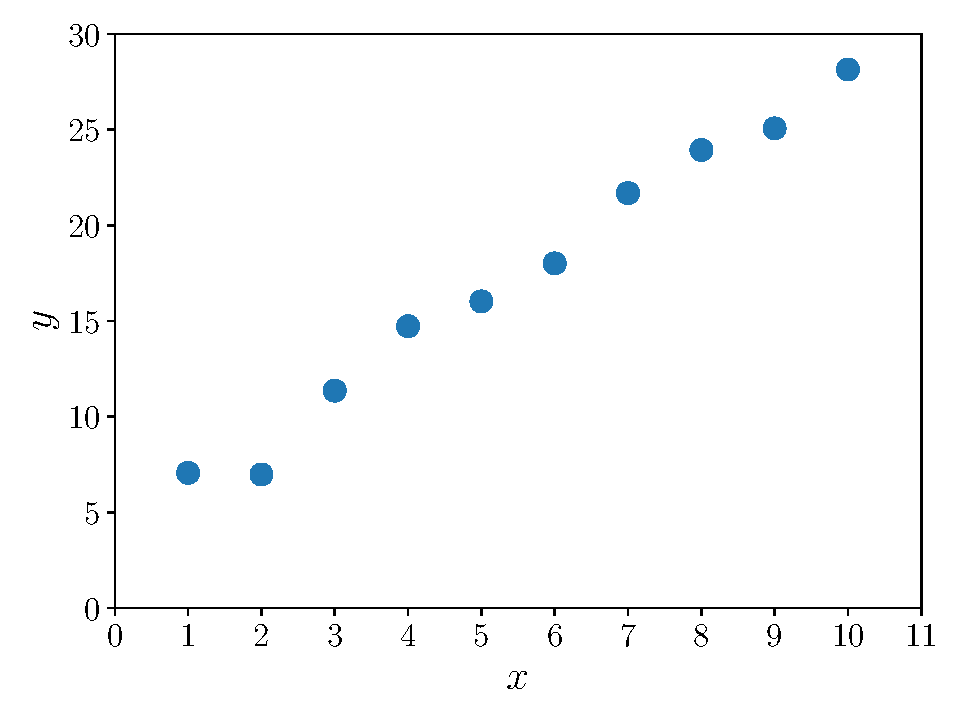
\includegraphics[width=1.0\textwidth]{figs/fig-01.pdf}
\end{center} \pause

\cx 
\begin{theorem}[]
Sea $f(t, y)$ definida en un conjunto convexo $D \in \R^2$. Si existe una constante $L > 0$ tal que
\[ \abs{ \frac{\partial f(t, y)}{\partial y} } \leq L, \; \forall (t, y) \in D \]
entonce $f$ satisface una condición de Lipschitz sobre $D$ en la variable $y$ con constante de Lipschitz $L$.
\end{theorem} \pause

\begin{theorem}[]
    Sea $D = \{(t, y) \,|\, t_0 \leq t \leq T \text{ y } -\infty < y < \infty \}$, y $f(t, y)$ continua en $D$. Si $f$ satisface una condición de Lipschitz sobre $D$ en la variable $y$, entonces el problema de valor inicial:
    \[ \begin{system} y'(t) = f(t, y), \; t_0 \leq T \leq b \\  y(t_0) = y_0 \end{system} \]

    tiene una solución única $y(t)$ para $t_0 \leq t \leq T$.
\end{theorem}
\end{columns}
\end{frame}

\begin{frame}
%En el ámbito del cálculo numérico, la expresión "well-posed problems" se traduce generalmente como "problemas bien planteados" o "problemas bien formulados". Un problema bien planteado en este contexto se refiere a un problema matemático que cumple con ciertas propiedades fundamentales que garantizan la existencia, unicidad y estabilidad de la solución. Estas propiedades son:

%1. Existencia: Significa que el problema tiene al menos una solución.

%2. Unicidad: Significa que el problema tiene una única solución, es decir, no tiene múltiples soluciones válidas.

%3. Estabilidad: Significa que pequeñas variaciones en los datos de entrada del problema no generan cambios drásticos en la solución, lo que implica que la solución es sensible de manera continua a las perturbaciones en los datos iniciales.

%Cuando un problema cumple con estas tres propiedades, se considera bien planteado en el contexto de cálculo numérico. Los problemas bien planteados son más adecuados para ser resueltos mediante métodos numéricos, ya que proporcionan una base sólida para obtener soluciones numéricas confiables y estables.
\begin{columns}[t]
\cx
\textbf{Problema bien formulado:}
\begin{itemize}
    \item Existencia: el problema tiene al menos una solución.
    \item Unicidad: el problema tiene solución única.
    \item Estabilidad: pequeñas variaciones en los datos de entrada no generan grandes cambios en la solución. 
\end{itemize} \pause

El problema de valor inicial:
\[ \begin{system} y'(t) = f(t, y), \; t_0 \leq t \leq T \\ y(t_0) = y_0 \end{system} \]
está bien formulado si:
\begin{itemize}
    \item Existe una solución única $y(t)$, y
    \item Existen constantes $\varepsilon_0 > 0$ y $k > 0$ tales que para cada cualquier $\varepsilon \in(0, \varepsilon_0)$, siempre que $\delta(t)$ sea continua con $\abs{\delta(t)} < \varepsilon, \; \forall t \in [t_0, T]$, y cuando $\abs{\delta_0} < \varepsilon$, el problema de valor inicial:
\end{itemize}

\cx
        \[ \begin{system} z'(t) = f(t, z) + \delta (t), \; t_0 \leq t \leq T \\ z(t_0) = y_0 + \delta_0 \end{system}\]
tiene una solución única que satisface
\[ \abs{z(t) - y(t)} < k \varepsilon, \; \forall t \in [t_0, T] \]

\begin{theorem}
Sea $D = \{(t, y) \,|\, t_0 \leq t \leq T \text{ y } -\infty < y < \infty \}$. Si $f$ es continua y satisface una condición de Lipschitz en la variable $y$ sobre el conjunto $D$, el problema de valor inicial:
\[ \begin{system} y'(t) = f(t, y), \; t_0 \leq t \leq T \\ y(t_0) = y_0 \end{system} \] 
está bien formulado.
\end{theorem}
\end{columns}
\end{frame}

\begin{frame}
\begin{columns}[t]
\vspace{1em}
\cx
\textbf{Serie de Taylor}: $f \in C^{(\infty)}$
 \begin{multline*} f(t) = f(t_0) + \frac{f'(t_0)}{1!} (t - t_0) + \frac{f''(t_0)}{2!} (t - t_0)^2 \\ + \frac{f^{(3)}(t_0)}{3!} (t - t_0)^3 + \cdots \end{multline*}   \pause
 \vspace{-2em}
 \begin{theorem}[Teorema de Taylor]
     Sea $k \geq 1$ un entero y $f: \R \mapsto \R$ $k$ veces diferenciable en $t_0 \in \R$. Entonces existe $h_k : \R \mapsto \R$ tal que: \vspace{-1em}
 \begin{multline*} f(t) = f(t_0) + \frac{f'(t_0)}{1!} (t - t_0) + \frac{f''(t_0)}{2!} (t - t_0)^2 \\ + \frac{f^{(3)}(t_0)}{3!} (t - t_0)^3 + \dots + \frac{f^{(k)}(t_0)}{k!} (t - t_0)^k \\+ h_k(t) (t-t_0)^k \end{multline*}
 y 
 \[ \lim_{t \to t_0} h_k(t) = 0 \]
\end{theorem}
\pause

\cx 
\textbf{Forma de Lagrange para el resto:} Sea $f: \R \to \R$ $k+1$ veces diferenciable en $(t_0, t)$ con $f^{(k)}$ continua en ${t_0, t}$:
\[ R_k(t) = \frac{f^{(k+1)}(\tau)}{(k+1)!} (t - t_0)^{k+1} \]
para $t_0 \leq \tau \leq t$. \pause
\vspace{1em}

\textbf{Método de Euler:}
$h = t_1 - t_0, y'(t) = f(t, y)$
\begin{align*}
    y_1 = y(t_1) &= y(t_0) + y'(t_0) (t_1 -t_0) + \frac{y''(\tau)}{2} (t_1 - t_0)^2 \\
                 &= y_0 + h f[t_0, y(t_0, y_0)] + y''(\tau) \frac{h^2}{2}
\end{align*}
\begin{itemize}
\item Aproximación: $y_1 = y_0 + h f(t_0, y_0)$
\item Error local: $\bigO(h^2)$
\item Error global: $\bigO(h)$
\end{itemize}
\end{columns}
\end{frame}

\begin{frame}
    \textbf{Método de Taylor:} $y$ tiene $n+1$ derivadas continuas en $[t_0, T]$, expansión de Taylor alrededor de $t_i$:
    \[ y(t) = y_0 + y'_i (t-t_i) + \frac{y''_i}{2}(t-t_i)^2 + \cdots + \frac{y^{(n)}_i}{n!} (t-t_i)^n + \frac{y^{(n+1)}(\tau)}{(n+1)!} (t-t_i)^{n+1} \]
\begin{align*}
    y'_i &= f(t_i, y_i) \\
    y''_i &= \left. \frac{d}{dt} f(t, y) \right|_{t = t_i} = \left. \left(\frac{\partial f}{\partial t} + \frac{\partial f}{\partial y} f \right) \right|_{t = t_i} \\
    y'''_i &= \left. \frac{d^2}{dt^2} f(t, y) \right|_{t = t_i} = \left. \left( \frac{\partial^2f}{\partial t^2} + 2 f \frac{\partial^2 f}{\partial t \partial y} + \frac{\partial^2 f}{\partial y^2} f^2 + \frac{\partial f}{\partial y} \frac{\partial f}{\partial t} + \left(\frac{\partial f}{\partial y} \right)^2 f \right) \right|_{t=t_i}
\end{align*}
Evaluando en $t=t_{i+1}$, descartando el resto y haciendo $h = t_{i+1} - t_i$:
\[ y_{i+1} = y_i + h f(t_i, y_i) + \frac{h^2}{2} \left. \frac{d}{dt} f(t, y) \right|_{(t_i, y_i)} + \cdots + \frac{h^n}{n!} \left. \frac{d^{n-1}}{dt^{n-1}} f(t, y) \right|_{(t_i, y_i)} \] 
        
        {\centering \alert{Nota:} el método de Euler es el de Taylor con $n = 1$. }
\end{frame}

\begin{frame}
\begin{columns}[t]
\cx
\textbf{Runge-Kutta de segundo orden}
\[
    \begin{system}
        y' = f(t, y), \; t_0 \leq t \leq T \\
        y(t_0) = y_0
    \end{system}
\]
\[ y_{n+1} = y_n + \int_{t_n}^{t_{n+1}} f(t, y) \, dt \]
Regla del trapecio:
\[ \int_{t_n}^{t_{n+1}} f(t, y) \, dt \simeq \frac{h}{2} [f(t_n, y_n) + f(t_{n+1}, y_{n+1})] \] 
Aproximamos:
\begin{align*}
    y_{n+1} \approx \lbar{y}_{n+1} &= y_n + h f(t_n, y_n) \\
    y_{n+1} &= y_n + \frac{h}{2} [f(t_n, y_n) + f(t_{n+1},\lbar{y}_{n+1})]
\end{align*}

\cx
Forma canónica:
\begin{align*}
    k_1 &= hf(t_n, y_n) \\
    k_2 &= h f(t_{n+1}, y_n + k_1) \\
    y_{n+1} &= y_n + \frac{1}{2} (k_1 + k_2)
\end{align*}

Errores:
\begin{itemize}
    \item Error local: $\bigO(h^3)$
    \item Error global $\bigO(h^2)$
\end{itemize}

RK2 óptimo (minimiza coeficiente de error): %% VERIFICAR EXPRESIONES !!
\begin{align*}
    k_1 &= \frac{2}{3} h f(t_i, y_i) \\
    k_2 &= \frac{3}{4} h f(t_i + \tfrac{2h}{3}, k_1) \\
    y_{n+1} &= y_n + \frac{1}{4} \left(\tfrac{3}{2} k_1 + 4 k_2\right)
\end{align*}
\end{columns}
\end{frame}

\begin{frame}
\begin{columns}[t]
\cw{0.4}
\textbf{Runge-Kutta de cuarto orden}
\[
    \begin{system}
        y' = f(t, y), \; t_0 \leq t \leq T \\
        y(t_0) = y_0
    \end{system}
\]
\[ y_{n+1} = y_n + \frac{1}{6} (k_0 + 2 k_1 + 2 k_2 + k_3) \]
con 
\begin{align*}
    k_0 &= h f(t_n, y_n) \\
    k_1 &= h f \left(t_n + \frac{h}{2}, y_n + \frac{k_0}{2}\right) \\
    k_2 &= h f \left(t_n + \frac{h}{2}, y_n + \frac{k_1}{2}\right) \\
    k_3 &= h f \left(t_n + h, y_n + k_2  \right) 
\end{align*} 
Errores:
\begin{itemize}
    \item Error local: $\bigO(h^5)$
    \item Error global $\bigO(h^4)$
\end{itemize}

\cw{0.55}
\textbf{Nota:} %% Alex Gezerlis
    Si $f(t, y) = f(t)$: integración de $1/3$ de Simpson
        \[ y_{n+1} = y_n + \frac{h}{6} \left[ f(x_n) + 4 f(x_n + \tfrac{h}{2}) + f(t_{n+1}) \right] \]  \pause

\textbf{Sistema de ecuaciones:}
\[ \begin{system} \bm{y}'(t) = \bm{f}(t, \bm{y}(t)) \\ \bm{y}(t_0) = \bm{y}_0 \end{system} \]
\begin{columns}[t]
\cw{0.4}
Euler:
\[ \bm{y}_{n+1} = \bm{y}_n + h \bm{f}(t_n, \bm{y}_n) \]

\cw{0.6}
RK4:
\begin{align*}
    \bm{k}_0 &= h \bm{f}(t_n, \bm{y}_n) \\
    \bm{k}_1 &= h \bm{f} \left(t_n + \frac{h}{2}, \bm{y}_n + \frac{\bm{k}_0}{2}\right) \\
        \bm{k}_2 &= h \bm{f} \left(t_n + \frac{h}{2}, \bm{y}_n + \frac{\bm{k}_1}{2}\right) \\
        \bm{k}_3 &= h \bm{f} \left(t_n + h, \bm{y}_n + \bm{k}_2  \right)
\end{align*} 
\[ \bm{y}_{n+1} = \bm{y}_n + \frac{1}{6} (\bm{k}_0 + 2 \bm{k}_1 + 2 \bm{k}_2 + \bm{k}_3) \]

\end{columns}
\end{columns}
\end{frame}

\begin{frame}[fragile]
\begin{columns}
\cw{0.45}
\pycode[firstline=2, lastline=26]{code/euler.py}

\cw{0.5}
\begin{center}
    \textbf{Euler hacia adelante}

    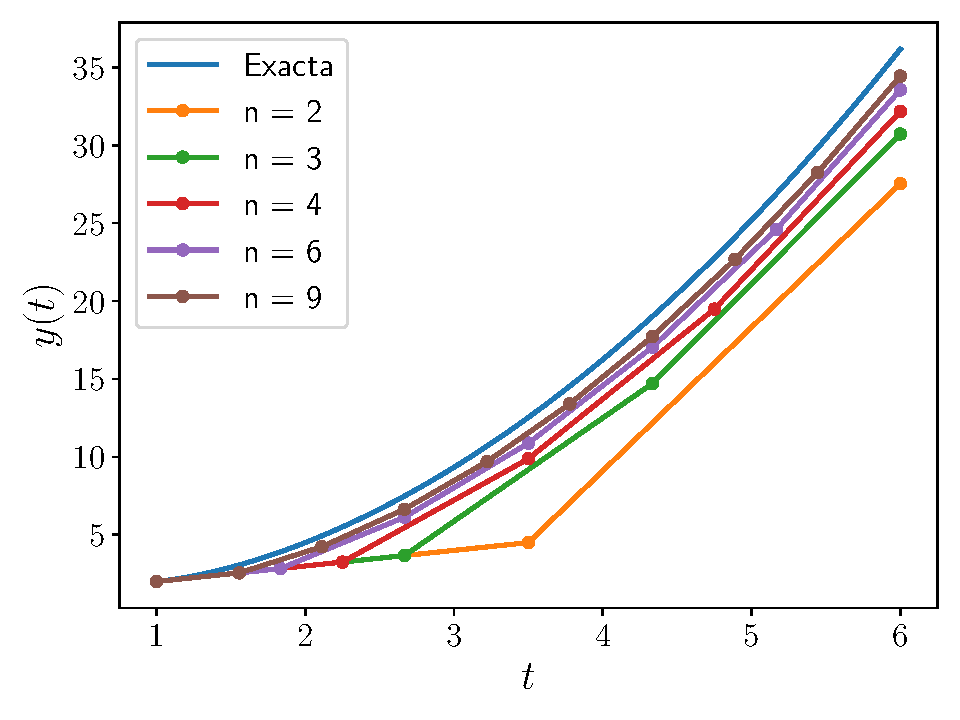
\includegraphics[width=0.9\textwidth]{code/euler.pdf}
\end{center}
\end{columns}
\end{frame}

\begin{frame}[fragile]
\begin{columns}
\cw{0.45}
\pycode[firstline=12, lastline=30]{code/rk4.py}

\cw{0.5}
\begin{center}
    \textbf{Runge-Kutta de cuarto orden}

    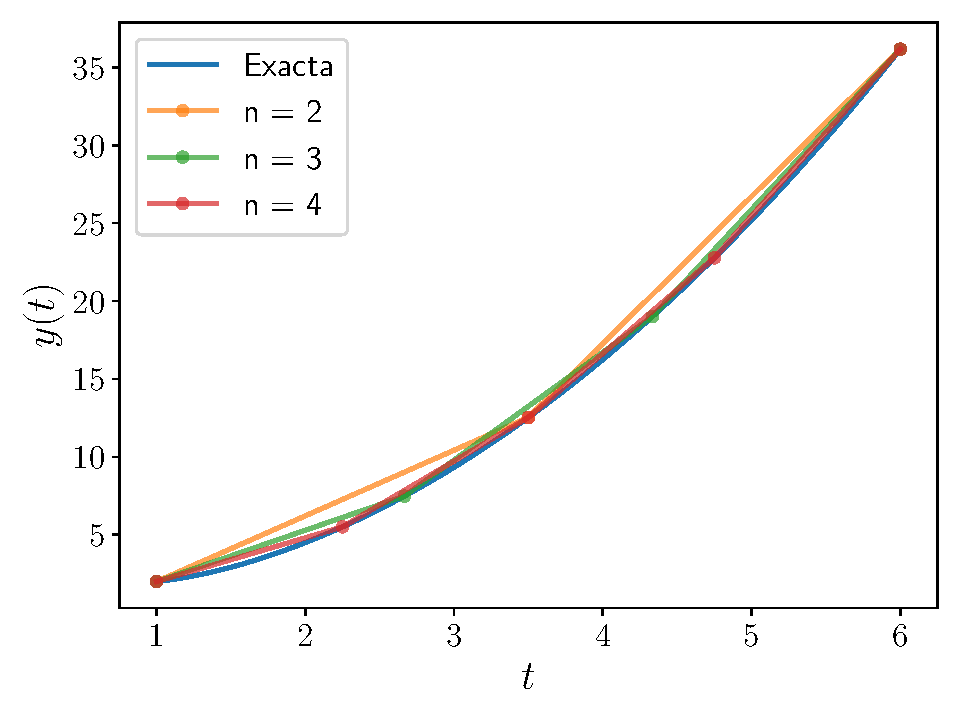
\includegraphics[width=0.9\textwidth]{code/rk4.pdf}
\end{center}
\end{columns}
\end{frame}

\begin{frame}[fragile]
\begin{columns}
\cw{0.45}
\pycode[firstline=12]{code/ivp.py}

\cw{0.5}
\begin{center}
    \textbf{\texttt{solve\_ivp} de SciPy}

    \includegraphics[width=0.9\textwidth]{code/solve_ivp.pdf}
\end{center}
\end{columns}
\end{frame}

\begin{frame}[fragile]
\begin{columns}
\cw{0.45}
\pycode{code/lotka-volterra.py}

\cw{0.5}
\begin{center}
    \textbf{Sistema Lotka-Volterra}
    \begin{align*}
        \frac{dx}{dt} &= \alpha x - \beta x y \\
        \frac{dy}{dt} &= \delta x y - \gamma y \\
        x(0) &= x_0, \, y(0) = y_0
    \end{align*}

    \includegraphics[width=0.9\textwidth]{code/lv.pdf}
\end{center}
\end{columns}
\end{frame}

\section*{Bibliografía}
\begin{frame}[allowframebreaks]{Lecturas recomendadas}
\begin{itemize}
    \item \fullcite{burden2017}. Capítulo 5.
    \item \fullcite{bradie2006}. Capítulo 7.
    \item \fullcite{gezerlis2020}. Capítulo 8.
    \item \fullcite{kiusalaas2013}. Capítulo 7.
\end{itemize}
\end{frame}

\end{document}

